\begin{appendices}
    \chapter{Assets.json}    
    \label{app:assetsjson}
    \lstset{language=JSON}
    \begin{lstlisting}
    {
        "common": [{
            "src": "assets/language/PDALanguage.lp",
            "id": "language"
        }],
        "scenario_test_movie": [{
                "src": "assets/scenarios/scenario_test_movie/story.json",
                "id": "story_scenario_test_movie"
            },
            {
                "src": "assets/scenarios/scenario_test_movie/story.lp",
                "id": "story_scenario_test_movie.lp"
            }
        ],
        "scenario_test_movie_lazyLoad": [{
                "src": "assets/scenarios/scenario_test_movie/images/JF_Angry.jpg",
                "id": "JF_Angry_jpg"
            },
            {
                "src": "assets/scenarios/scenario_test_movie/images/JF_Angry.png",
                "id": "JF_Angry_png"
            },
            {
                "src": "assets/scenarios/scenario_test_movie/images/JF_Sad.jpg",
                "id": "JF_Sad_jpg"
            },
            {
                "src": "assets/scenarios/scenario_test_movie/images/JF_Sad.png",
                "id": "JF_Sad_png"
            }
        ],
        "sounds": [{
                "src": "assets/sounds/click.mp3",
                "id": "click"
            },
            {
                "src": "assets/sounds/counter_1.mp3",
                "id": "counter"
            },
            {
                "src": "assets/sounds/drill.mp3",
                "id": "drill"
            },
    
            {
                "src": "assets/sounds/pda/smartphone_open.mp3",
                "id": "smartphone_open"
            },
            {
                "src": "assets/sounds/pda/smartphone_close.mp3",
                "id": "smartphone_close"
            },
            {
                "src": "assets/sounds/pda/smartphone_clickbutton.mp3",
                "id": "smartphone_clickbutton"
            }
        ]
    }
    \end{lstlisting}

    \chapter{Voorbeeld content typen schema}
    \lstset{language=JSON}
    \begin{lstlisting}
    {
        "$schema": "http://json-schema.org/draft-07/schema#",
        "$id": "http://www.ranjnet.nl/ozcontent#",
        "title": "&ranj game content",
        "description": "This schema defines the content types within the game content",
        "definitions": {
            "propertyTypes": {
                "stringProperty": {
                    "$id": "#/definitions/propertyTypes/stringProperty",
                    "type": "string",
                    "default": ""
                },
                "booleanProperty": {
                    "$id": "#/definitions/propertyTypes/booleanProperty",
                    "type": "boolean",
                    "default": false
                },
                "resourceProperty": {
                    "$id": "#/definitions/propertyTypes/resourceProperty",
                    "type": "string"
                },
                "variableMutationProperty": {
                    "$id": "#/definitions/propertyTypes/variableMutationProperty",
                    "type": "object",
                    "properties": {
                        "variableKey": {
                            "$ref": "#/definitions/propertyTypes/stringProperty"
                        },
                        "mutationType": {
                            "$ref": "#/definitions/propertyTypes/stringProperty",
                            "enum": [
                                "Set",
                                "Add",
                                "Subtract",
                                "Multiple",
                                "Divide"
                            ],
                            "default": "Set"
                        },
                        "mutationValue": {
                            "$ref": "#/definitions/propertyTypes/stringProperty"
                        }
                    }
                }
            },
            "baseContent": {
                "type": "object",
                "properties": {
                    "contentType": {
                        "$ref": "#/definitions/propertyTypes/stringProperty"
                    },
                    "label": {
                        "$ref": "#/definitions/propertyTypes/stringProperty",
                        "title": "Label"
                    },
                    "retained": {
                        "$ref": "#/definitions/propertyTypes/booleanProperty",
                        "title": "Retained"
                    },
                    "contentID": {
                        "$ref": "#/definitions/propertyTypes/stringProperty",
                        "title": "Content ID"
                    }
                },
                "required": [
                    "type",
                    "label",
                    "retained",
                    "contentID"
                ]
            }
        },
        "contentTypes": {
            "textContent": {
                "allOf": [{
                        "$ref": "#/definitions/baseContent"
                    },
                    {
                        "$id": "#/contentTypes/textContent",
                        "title": "Text content",
                        "description": "Textual content",
                        "properties": {
                            "text": {
                                "allOf": [{
                                        "$ref": "#/definitions/propertyTypes/stringProperty"
                                    },
                                    {
                                        "title": "Text",
                                        "description": "Value of the textual content"
                                    }
                                ]
                            }
                        }
                    }
                ]
            },
            "imageContent": {
                "allOf": [{
                        "$ref": "#/definitions/baseContent"
                    },
                    {
                        "$id": "#/contentTypes/imageContent",
                        "title": "Image content",
                        "properties": {
                            "imageResource": {
                                "allOf": [{
                                        "$ref": "#/definitions/propertyTypes/resourceProperty"
                                    },
                                    {
                                        "assetType": "image"
                                    }
                                ]
                            }
                        }
                    }
                ]
            },
            "variableMutationContent": {
                "allOf": [{
                        "$ref": "#/definitions/baseContent"
                    },
                    {
                        "title": "Mutate variable content",
                        "$id": "#/contentTypes/variableMutationContent",
                        "properties": {
                            "mutations": {
                                "type": "array",
                                "items": {
                                    "$ref": "#/definitions/propertyTypes/variableMutationProperty"
                                }
                            }
                        }
                    }
                ]
            }
        }
    }
    \end{lstlisting}
    
    \chapter{Use cases voor een overkoepelende projectstructuur}
    \label{app:usecasesprojectstructuur}
    \begin{itemize}
        \item Als gebruiker wil ik kunnen kiezen uit een lijst van (gecategoriseerde) assets.
        \item Als gebruiker wil ik gewaarschuwd worden als ik een niet-bestaande of verkeerd type asset gebruik.
        \item Als gebruiker wil ik een preview kunnen zien of horen als mogelijk.
        \item Als gebruiker wil ik assets kunnen openen. (dialog/ story files openen in de editor, afbeeldingen met default afbeeldingen programma)
        \item Als gebruiker wil ik dat mijn game geen ongebruikte assets laadt. (Als speler wil ik dat mijn game snel laad).
    \end{itemize}

    \chapter{Balkenplanning}
    \label{app:ganttchart}
    \newgantttimeslotformat{stardate}{%
        \def\decomposestardate##1.##2\relax{%
        \def\stardateyear{##1}\def\stardateday{##2}%
        }%
        \decomposestardate#1\relax%
        \pgfcalendardatetojulian{\stardateyear-01-01}{#2}%

        \advance#2 by-1\relax%
        \advance#2 by\stardateday\relax%
    }

    \newcounter{myWeekNum}
    \stepcounter{myWeekNum}
    
    \newcommand{\myWeek}{\themyWeekNum
        \stepcounter{myWeekNum}
        \ifnum\themyWeekNum=6
            \setcounter{myWeekNum}{1}
        \else\fi
    }

    \setcounter{myWeekNum}{6}
    \ganttset{%
        calendar week text={\myWeek{}}%
    }

    \begin{landscape}
        \begin{ganttchart}[
            hgrid,
            vgrid,
            time slot format=stardate
            ]{2018.36}{2018.168} % year.daynumber
            \gantttitlecalendar{year, month=name, week} \\
            \ganttbar{Wat wordt er verstaan onder flexibel?}{2018.50}{2018.80} \\
            \ganttbar{In kaart brengen huidige narrative framework}{2018.36}{2018.50} \\
            \ganttbar{Zijn er al bestaande oplossingen die aansluiten bij de requirements?}{2018.80}{2018.168} \\
            \ganttbar{Onderzoek: Welke frameworks/ libraries/ tools zijn er en zijn inzetbaar?}{2018.80}{2018.168} \\
            \ganttbar{Inlezen libraries}{2018.80}{2018.168} \\
            \ganttbar{Boilerplate opzetten met frameworks}{2018.80}{2018.168} \\
            \ganttbar{In kaart brengen (project specifieke) configuraties van de huidige bewerkers + gewenste nieuwe configuraties}{2018.80}{2018.168} \\
            \ganttbar{Hoe maken we deze project specifieke configuraties configureerbaar per project?}{2018.80}{2018.168} \\
            \ganttbar{Waaruit bestaat 'game content'}{2018.80}{2018.168} \\
            \ganttbar{Onderzoek naar asset management}{2018.80}{2018.168} \\
            \ganttbar{Hoe kan er semantiek aan assets verbonden worden?}{2018.80}{2018.168} \\
            \ganttbar{Onderzoek: Welke formalismen zijn er?}{2018.80}{2018.168} \\
            \ganttbar{Hoe kunnen we het narrative editor framework future-proof maken op het gebied van formalismen?}{2018.80}{2018.168} \\
            \ganttbar{Prototype maken ter onderbouwing van het advies op ondersteuning voor verschillende formalismen.}{2018.80}{2018.168} \\
        \end{ganttchart}
    \end{landscape}

    \chapter{Content typen dataschema in XML}
    \label{app:contenttypeschemeinxml}
    % \subsection*{XML-dataschema}
    XML heeft al ingebouwde dataschema functionaliteit; de onderliggende structuur van een XML-object kan worden gespecificeerd. Dit bereikt XML door middel van elementen en attributen. Zo kan ‘sms content’ worden beschreven in een XML-dataschema als in \autoref{fig:xmlschemasmscontent}. Vervolgens kunnen XML-objecten gevalideerd worden door het schema. Het XML-object in \autoref{fig:xmlsmscontent} is valide, want de structuur komt overeen met die van het dataschema in \autoref{fig:xmlschemasmscontent}.

    \begin{figure}[htb]
        \centering
        \lstset{
        language=XML,
        morekeywords={encoding,
            xs:schema,xs:element,xs:complexType,xs:sequence,xs:attribute}
        }
        \begin{lstlisting}
        <?xml version="1.0" encoding="UTF-8"?>
        <xs:schema xmlns:xs="http://www.w3.org/2001/XMLSchema">
            <xs:element name="smscontent">
                <xs:complexType>
                    <xs:sequence>
                        <xs:element name="sender" type="xs:string" />
                        <xs:element name="receiveDate" type="xs:dateTime" />
                        <xs:element name="content" type="xs:string" />
                    </xs:sequence>
                </xs:complexType>
            </xs:element>
        </xs:schema>                
        \end{lstlisting}
        \caption{XML-dataschema voor 'sms content'.}
        \label{fig:xmlschemasmscontent}
    \end{figure}

    \begin{figure}[htb]
        \centering
        \lstset{language=XML}
        \begin{lstlisting}[firstnumber=1]
        <?xml version="1.0" encoding="UTF-8"?>
        <smscontent>
            <sender>Harold</sender>
            <receiveDate>2018-04-21T11:00:00</receiveDate>
            <content>Great moves, keep it up!</content>
        </smscontent>              
        \end{lstlisting}
        \caption{Valide XML-object van 'sms content'.}
        \label{fig:xmlsmscontent}
    \end{figure}

    % Getuigenverklaringen
    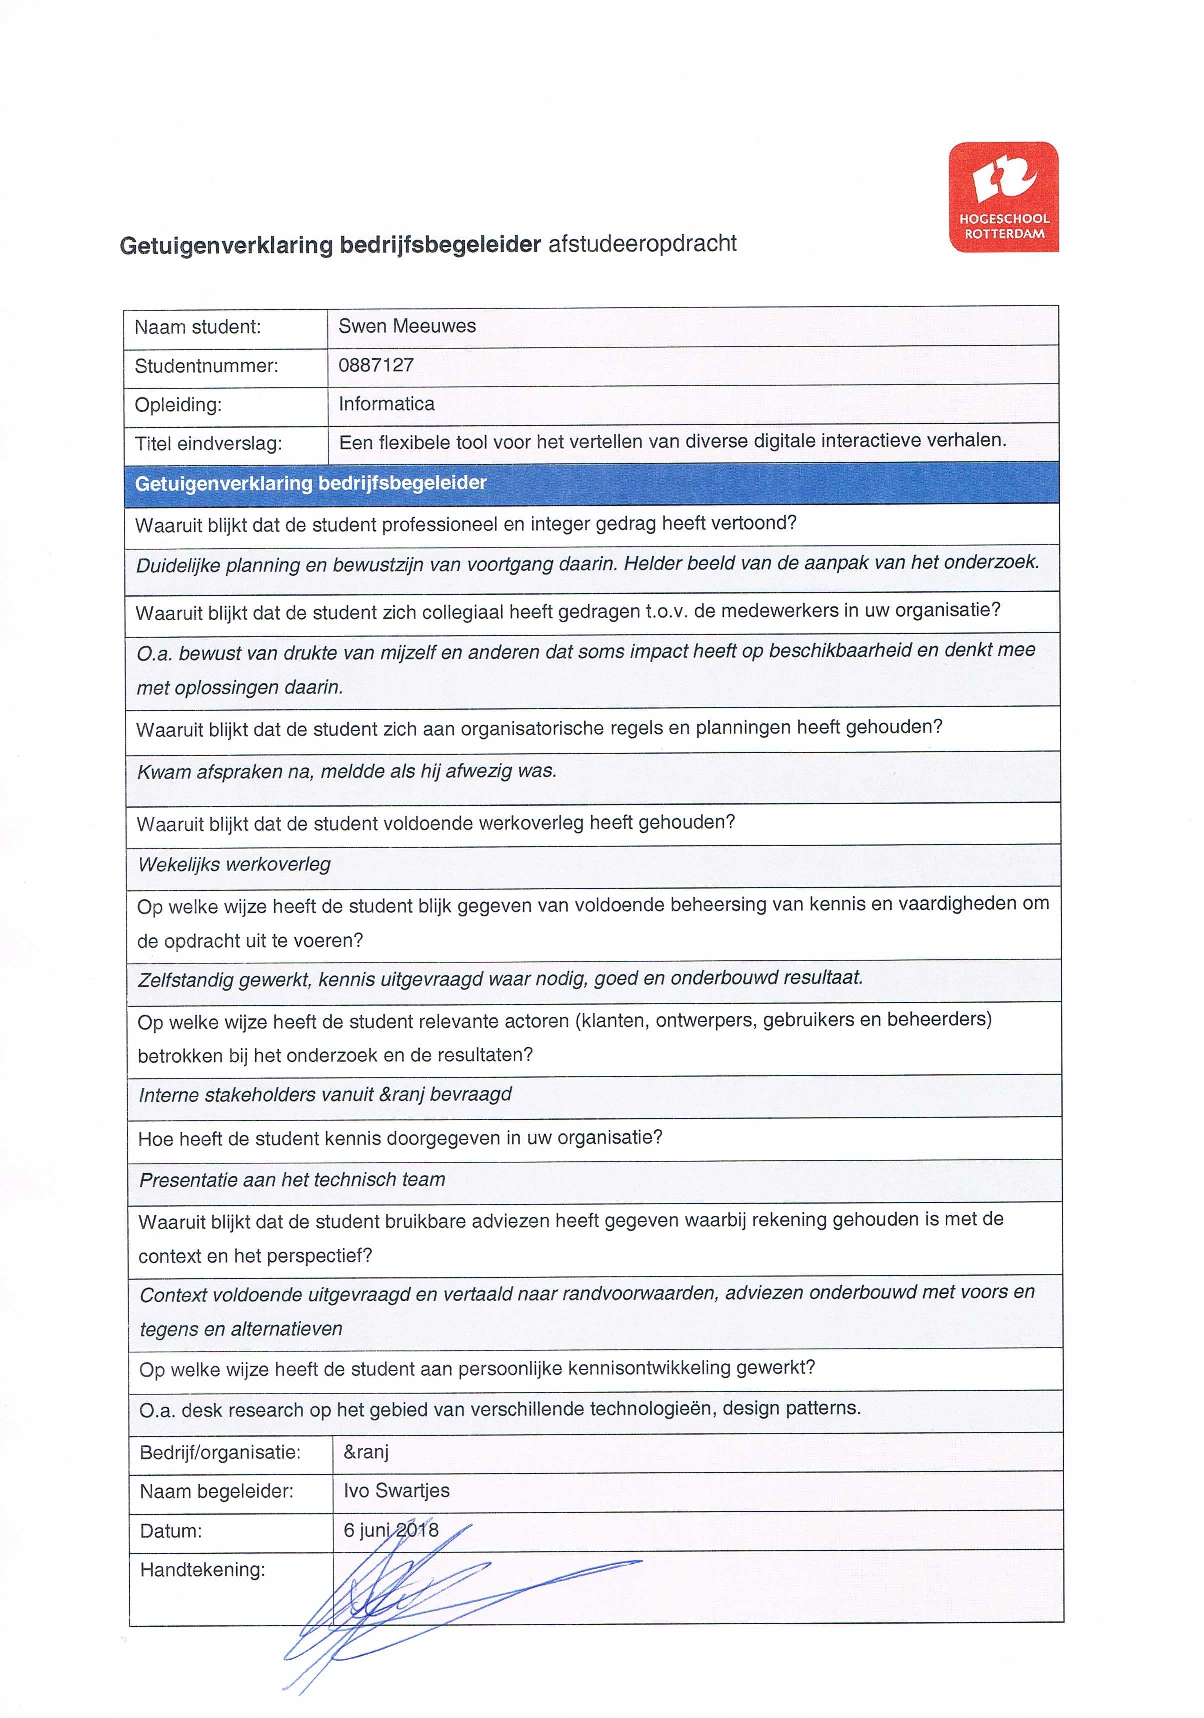
\includepdf[pages=-,scale=.75,offset=0mm -25mm,pagecommand=\chapter{Getuigenverklaringen}]{assets/pdf/Getuigenverklaring_bedrijfsbegeleider.pdf}
    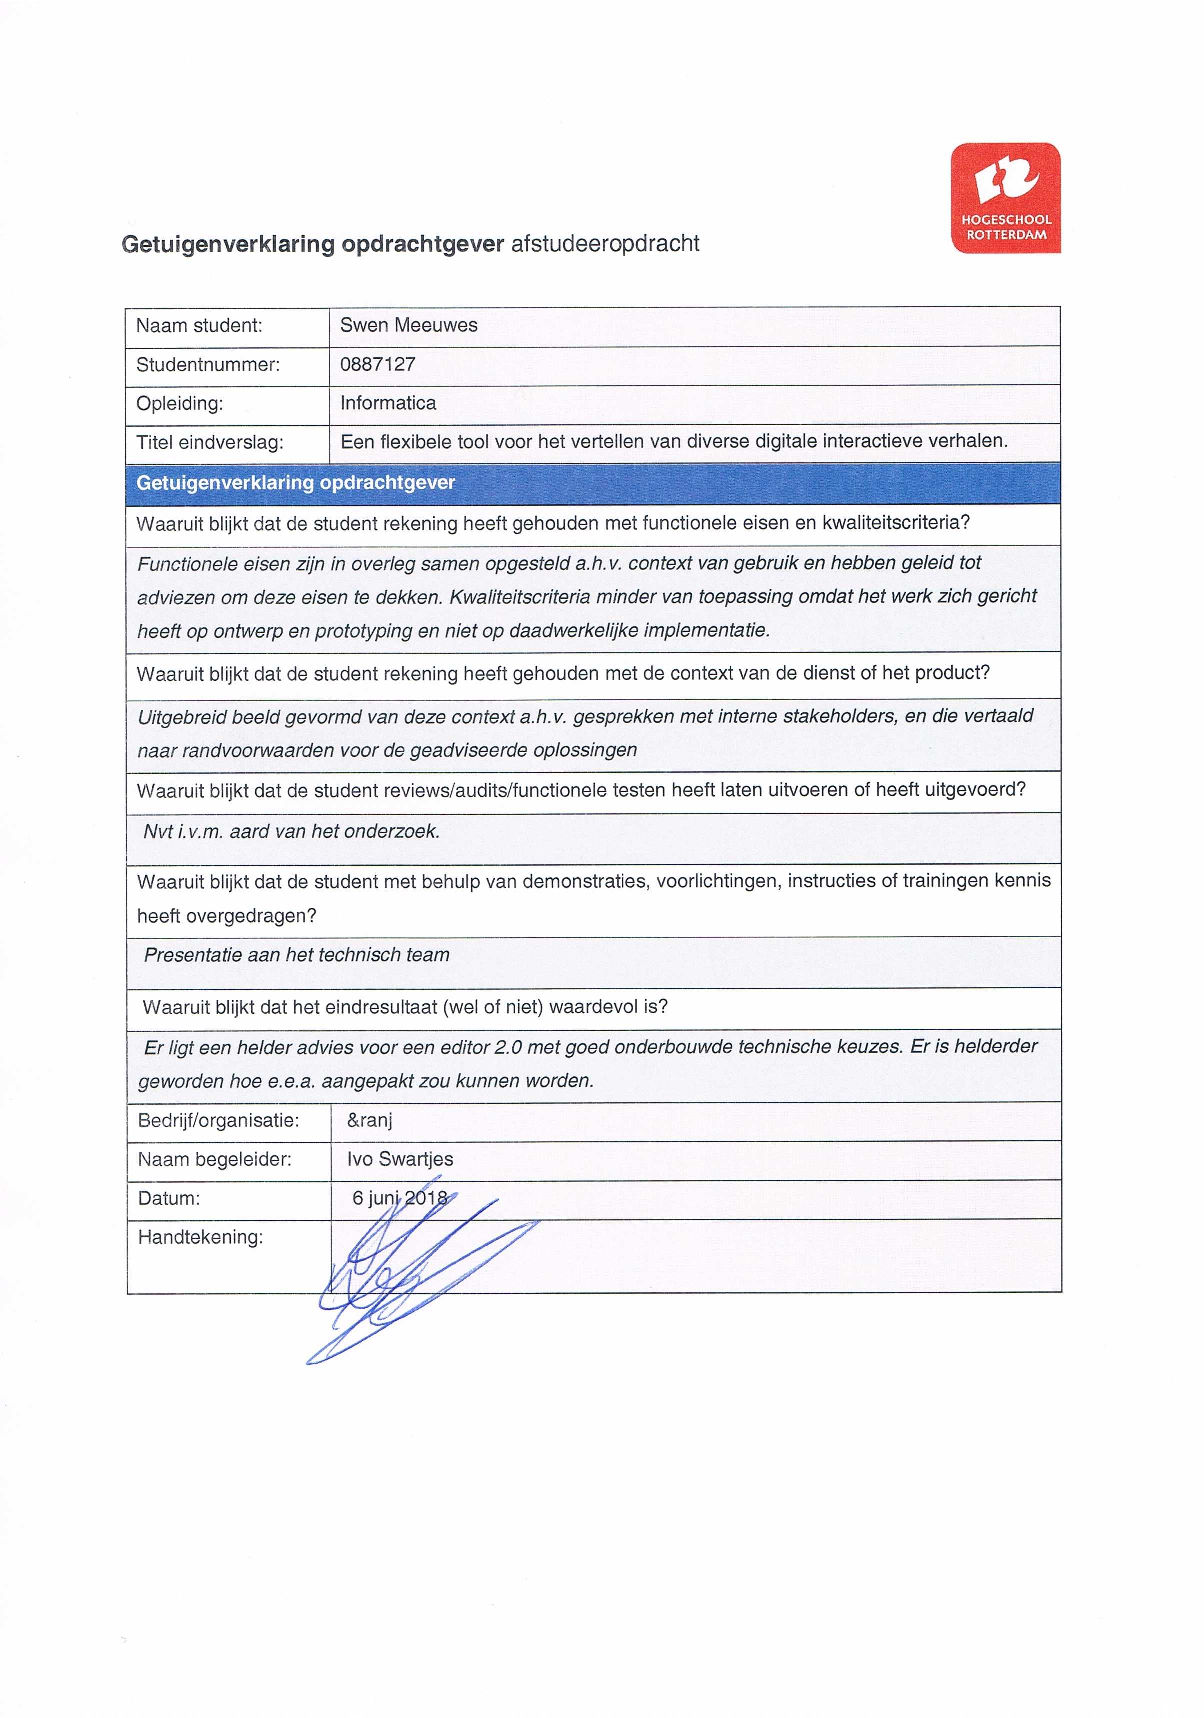
\includepdf[pages=-,scale=.75,pagecommand={}]{assets/pdf/Getuigenverklaring_opdrachtgever.pdf}
\end{appendices}